\documentclass[12pt]{article}
\usepackage[a4paper, text={6.5in,9in}]{geometry}
% \usepackage[utf8]{inputenc}
\usepackage{graphicx}
\graphicspath{ {images/} }

\usepackage{titling}

\usepackage{hyperref}
\hypersetup{
    colorlinks,
    citecolor=black,
    filecolor=black,
    linkcolor=black,
    urlcolor=black
}

% \usepackage{fancyhdr}
% \pagestyle{fancy}

\usepackage{amsmath}
\usepackage{amssymb}
\usepackage{mathtools}
\usepackage{dsfont}
\usepackage{cases}
% \newcommand*{\Z}{\mathds{Z}}

\usepackage{minted, xcolor}
%\usemintedstyle{monokai}
\definecolor{bg}{HTML}{F0F0F0}
% \usepackage[defaultmono]{droidsansmono}
% \usepackage[T1]{fontenc}

\newcommand{\nothing}{\text{\O}}

\newenvironment{code}[2][python]
{
    \VerbatimEnvironment
	\begin{listing}[H]%
		\caption{#2}%
        \begin{minted}[bgcolor=bg, breaklines, fontsize=\small, mathescape=true, escapeinside=||, linenos]{#1}%
}
{
		\end{minted}
	\end{listing}
}

% Code caption as 'Code: caption'
\renewcommand{\listingscaption}{Code}

\pretitle{%
   \begin{center}
   \LARGE
   
\includegraphics[width=6cm]{logo-unipd} \\ [\bigskipamount]
}
\posttitle{\end{center}}

\title{\textbf{Università di Padova \\ Formal Methods for Cyber-Physical Systems project report}}
\author{Alberto Lazari - 2089120 \\ Elia Scandaletti - 2087934 \\ Francesco Protopapa - 2079466 \\}
\date{January 2023 - A.Y. 2022-2023}

\begin{document}
    \maketitle
    \pagebreak

    \tableofcontents
    \pagebreak

    \section{Notation}
    \begin{description}
        \item $Post$: function which represents the set of states reachable from a given region by applying a single step of transition;
        \item $Pre$: function which represents the set of states from which a given state can be reached by applying a single step of transition;
        \item $List[i]$: element of list $List$ of index $
        \begin{cases}
            i, \mbox{if } i \geq 0 \\
            Size(List) + i, \mbox{if } i < 0
        \end{cases}, i \in \mathbb N$;
        \item $List[i:j]$: sublist of $List$ from index $i$ (included) to index $j$ (excluded). 
    \end{description}

    \section{Report Structure}
    In this report the problem is divided in two parts:
    \begin{itemize}
        \item deciding if the LTL formula is respected; 
        \item finding a witness in which the formula is not satisfied.
    \end{itemize}
    Each of these parts is discussed separately in its own section.

    \section{LTL Formula Satisfiability}
    \subsection{Algorithm Description}
    Since we are working with reactive formulas in the form $\square \diamondsuit F \implies \square \diamondsuit G$, we want to find whether exists a loop passing thorugh $F$ and avoiding $G$.
    For this reason, we will assume that $F \cap G = \nothing$; in case this doesn't hold we consider $F \leftarrow F \setminus G$.
    Furthermore we consider $G$ to be unreachable, i.e. whenever we applly the $Pre$ or $Post$ operations, we exclude $G$ from the result, unless otherwise specified.
    Lastly, we assume $F$ to be fully reachable; if this doesn't hold, we consider $F \leftarrow F \cap Reach$.

    The algorithm is composed of two nested loops.
    The inner one, given a region $Recur_i$, find the region $Recur_{i+1} \subseteq Recur_i$
    s.t. $Recur_{i+1}$ is the set of all and only states in $Recur_i$ from which $Recur_i$ is reachable.
    We start using $Recur_0 = F$

    This means that any potential loop passing through $Recur_i$ must pass through the $Recur_{i+1}$ region at least once.
    Therefore, any potential loop passing through $F$ must pass through the $Recur_{i+1}$ region at least once.
    
    In the outer loop we iteratively find such regions until either:
    \begin{itemize}
        \item $Recur_{i+1} = Recur_i$;
        \item $Recur_{i+1} = \nothing$.
    \end{itemize}
    In both cases $Recur$ is the last calculated region.

    In the former one, we know that for each state $s$ inside $Recur$ there exist a state $s'$ inside $Recur$ that can be reached from $s$ in one or more steps.
    Therefore there exists a path passing through $Recur$ infinitely many times.
    Since the number of states in $Recur$ is finite, some of these must repeat infinitely many times.
        
    In the latter case, no loop can pass through $F$ because no loop can pass through $Recur$.

    \subsection{Implementation}
    The implementation of the algorithm in pseudocode is the following:

    \begin{code}{pseudocode of the main function.}
function check_react_spec:
    |$F \leftarrow (F \cap Reach) \setminus G$|
    |$Recur \leftarrow F$|
    while |$Recur \neq \nothing$|:
        |$PreReach \leftarrow \nothing$|
        |$New \leftarrow Pre(Recur, Trans) \setminus G$|
        while |$New \neq \nothing$|:
            |$PreReach \leftarrow PreReach \cup New$|
            if |$Recur \subseteq PreReach$|:
                return False
            |$New \leftarrow (Pre(New, Trans) \setminus G) \setminus PreReach$|
        |$Recur \leftarrow Recur \cap PreReach$|
    return True
    \end{code}
    In case we find that $Recur \subseteq PreReach$, we can already say that we are in the case $Recur_{i+1} = Recur_i$, since $PreReach$ represents the regions of state from which is possible to reach $Recur_i$ in one or more steps.

    \noindent For the Python implementation, it is sufficient to translate the following instructions:
    \begin{itemize}
        \item $A \leftarrow B$ becomes: \mintinline{python}{A = B}
        \item $A \cap B$ becomes: \mintinline{python}{A & B}
        \item $A \setminus B$ becomes: \mintinline{python}{A - B}
        \item $A \neq \nothing$ becomes: \mintinline{python}{not A.is_false()}
        \item $Pre(A, Trans)$ becomes: \mintinline{python}{model.pre(A)}
        \item $A \cup B$ becomes: \mintinline{python}{A + B}
    \end{itemize}

    \section{Witness Search}
    \subsection{Algorithm Description}
    The algorithm is split in three main parts:
    \begin{description}
        \item[\texttt{partial\_loop\_trace}:] finds a list of states starting from a given state in $Recur$ and ending in $Recur$;
        \item[\texttt{loop\_trace}:] finds a loop starting and ending in the same state in $Recur$;
        \item[\texttt{init\_to\_s\_trace}:] finds a list of states describing a path from $Init$ to a given state.
    \end{description}
    Inside \texttt{init\_to\_s\_trace} we also consider states within region $G$.

    Beside, there are some utilities functions:
    \begin{description} 
        \item[\texttt{post\_reach}:] calculate the region of reachable states from a given region;
        \item[\texttt{desimbolify}:] given a list of regions returns a list of states in which:
        \begin{itemize}
            \item each state is inside the corrisponding region in the input list;
            \item each state is reachable in one step from the preceding one.
        \end{itemize}
        \item[\texttt{create\_trace}:] orchestrate the three main functions in order to build a witness;
        \item[\texttt{create\_trace\_inputs}:] given a list of states, it returns a list of alternating inputs and states representing a witness.
    \end{description}

    We are now going to illustrate the working of the main parts of the algorithm.

    \paragraph*{\texttt{partial\_loop\_trace}}
    This function iteratively computes the reachable region of a given state in $Recur$, meanwhile it builds a list of regions it is passing through.
    It stops as soon as it is able to reach a sub-region of $Recur$.
    Finally, it desimbolifies the trace it built and returns it.
    In doing so, the function is able to return a path starting in the given state and ending in $Recur$.

    \begin{figure}[H] 
        \centering
        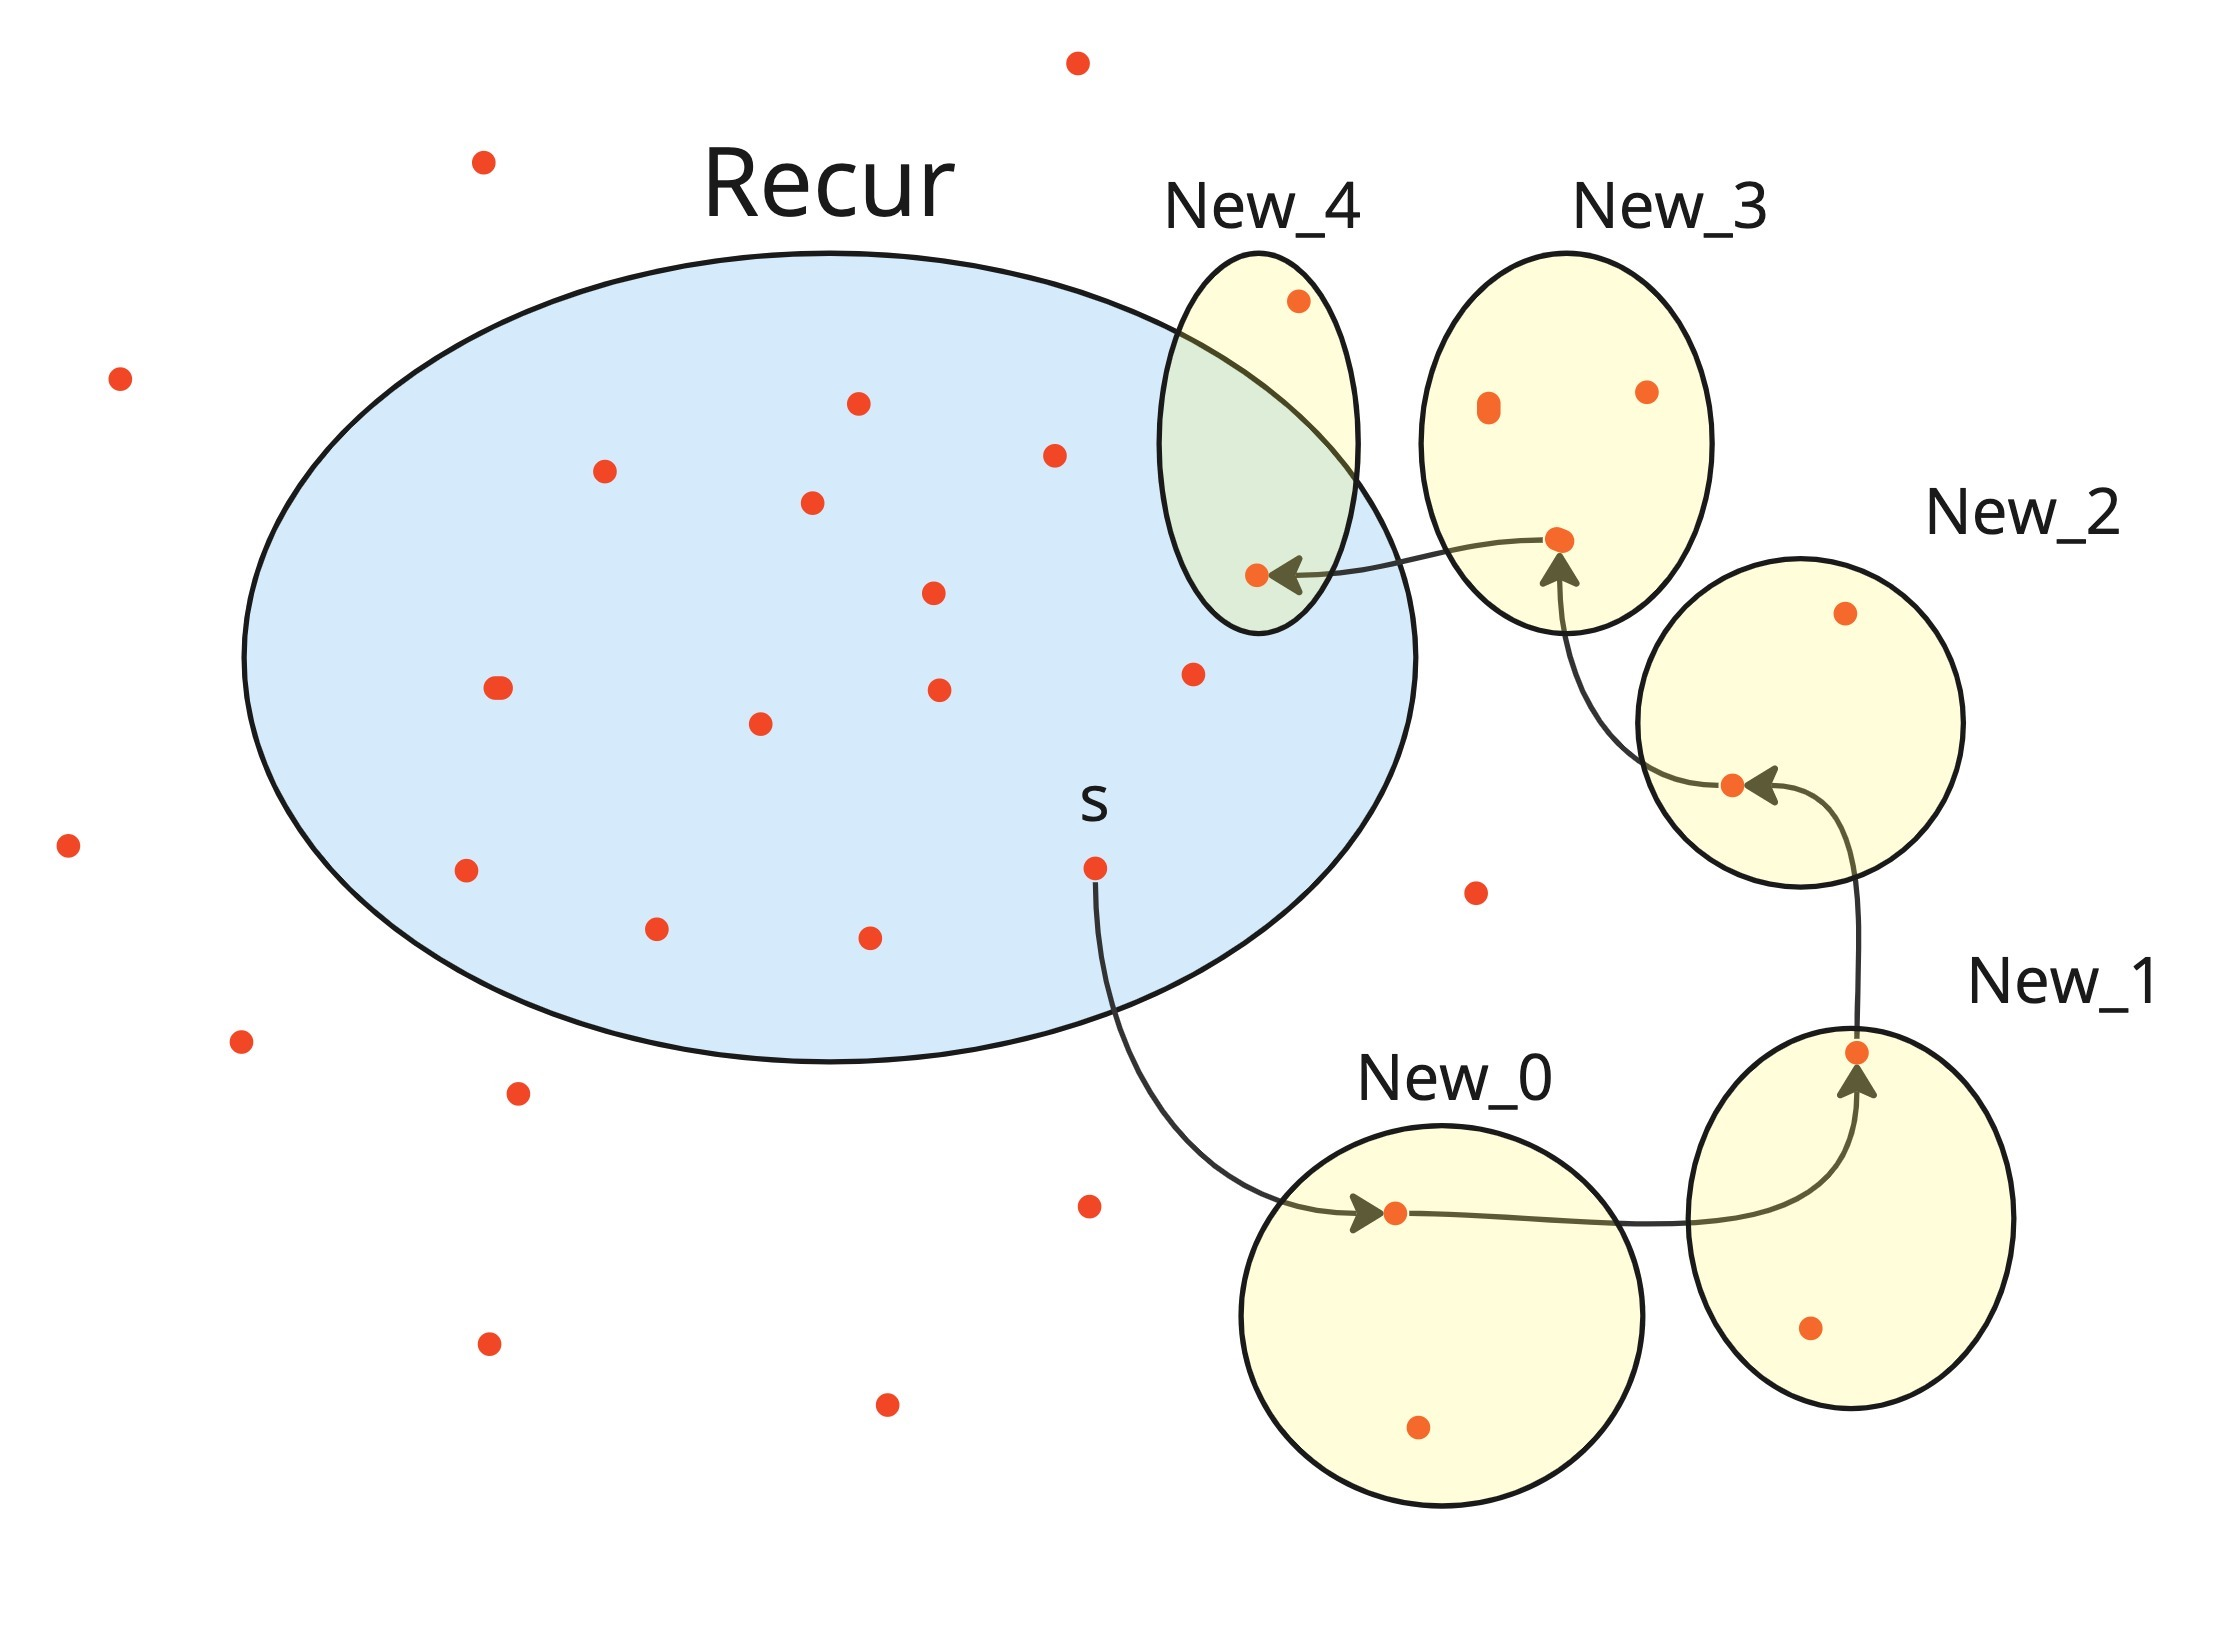
\includegraphics[width=0.6\textwidth]{partial_loop_trace.jpg}
        \caption{Representation of the \texttt{partial\_loop\_trace} algorithm.}
        \label{fig:partial_loop_trace}
    \end{figure}

    In Figure \ref{fig:partial_loop_trace} each red dot represents a state; each yellow region the region represented by $New$ at each iteration; each arrow represents one step.
            
    \paragraph*{\texttt{loop\_trace}}
    This function iteratively uses \texttt{partial\_loop\_trace} in order to build a loop starting and ending in $Recur$.
    It begins picking a state $s_0$ in $Recur$ and at each iteration uses \texttt{partial\_loop\_trace} to find a path $s_i$\dots$s_{i+1}$ ending in $Recur$.
    It concatenates all these subpaths until it finds a path ending in a state already visited.

    Lastly, it ``cleans'' the loop before retuning it.
    The loop could have a lasso shape so the function removes the leading subpath in order to return just a looping path.
    The loop is anyway granted to start inside $Recur$ since it's granted to end inside $Recur$.

    \begin{figure}[H] 
        \centering
        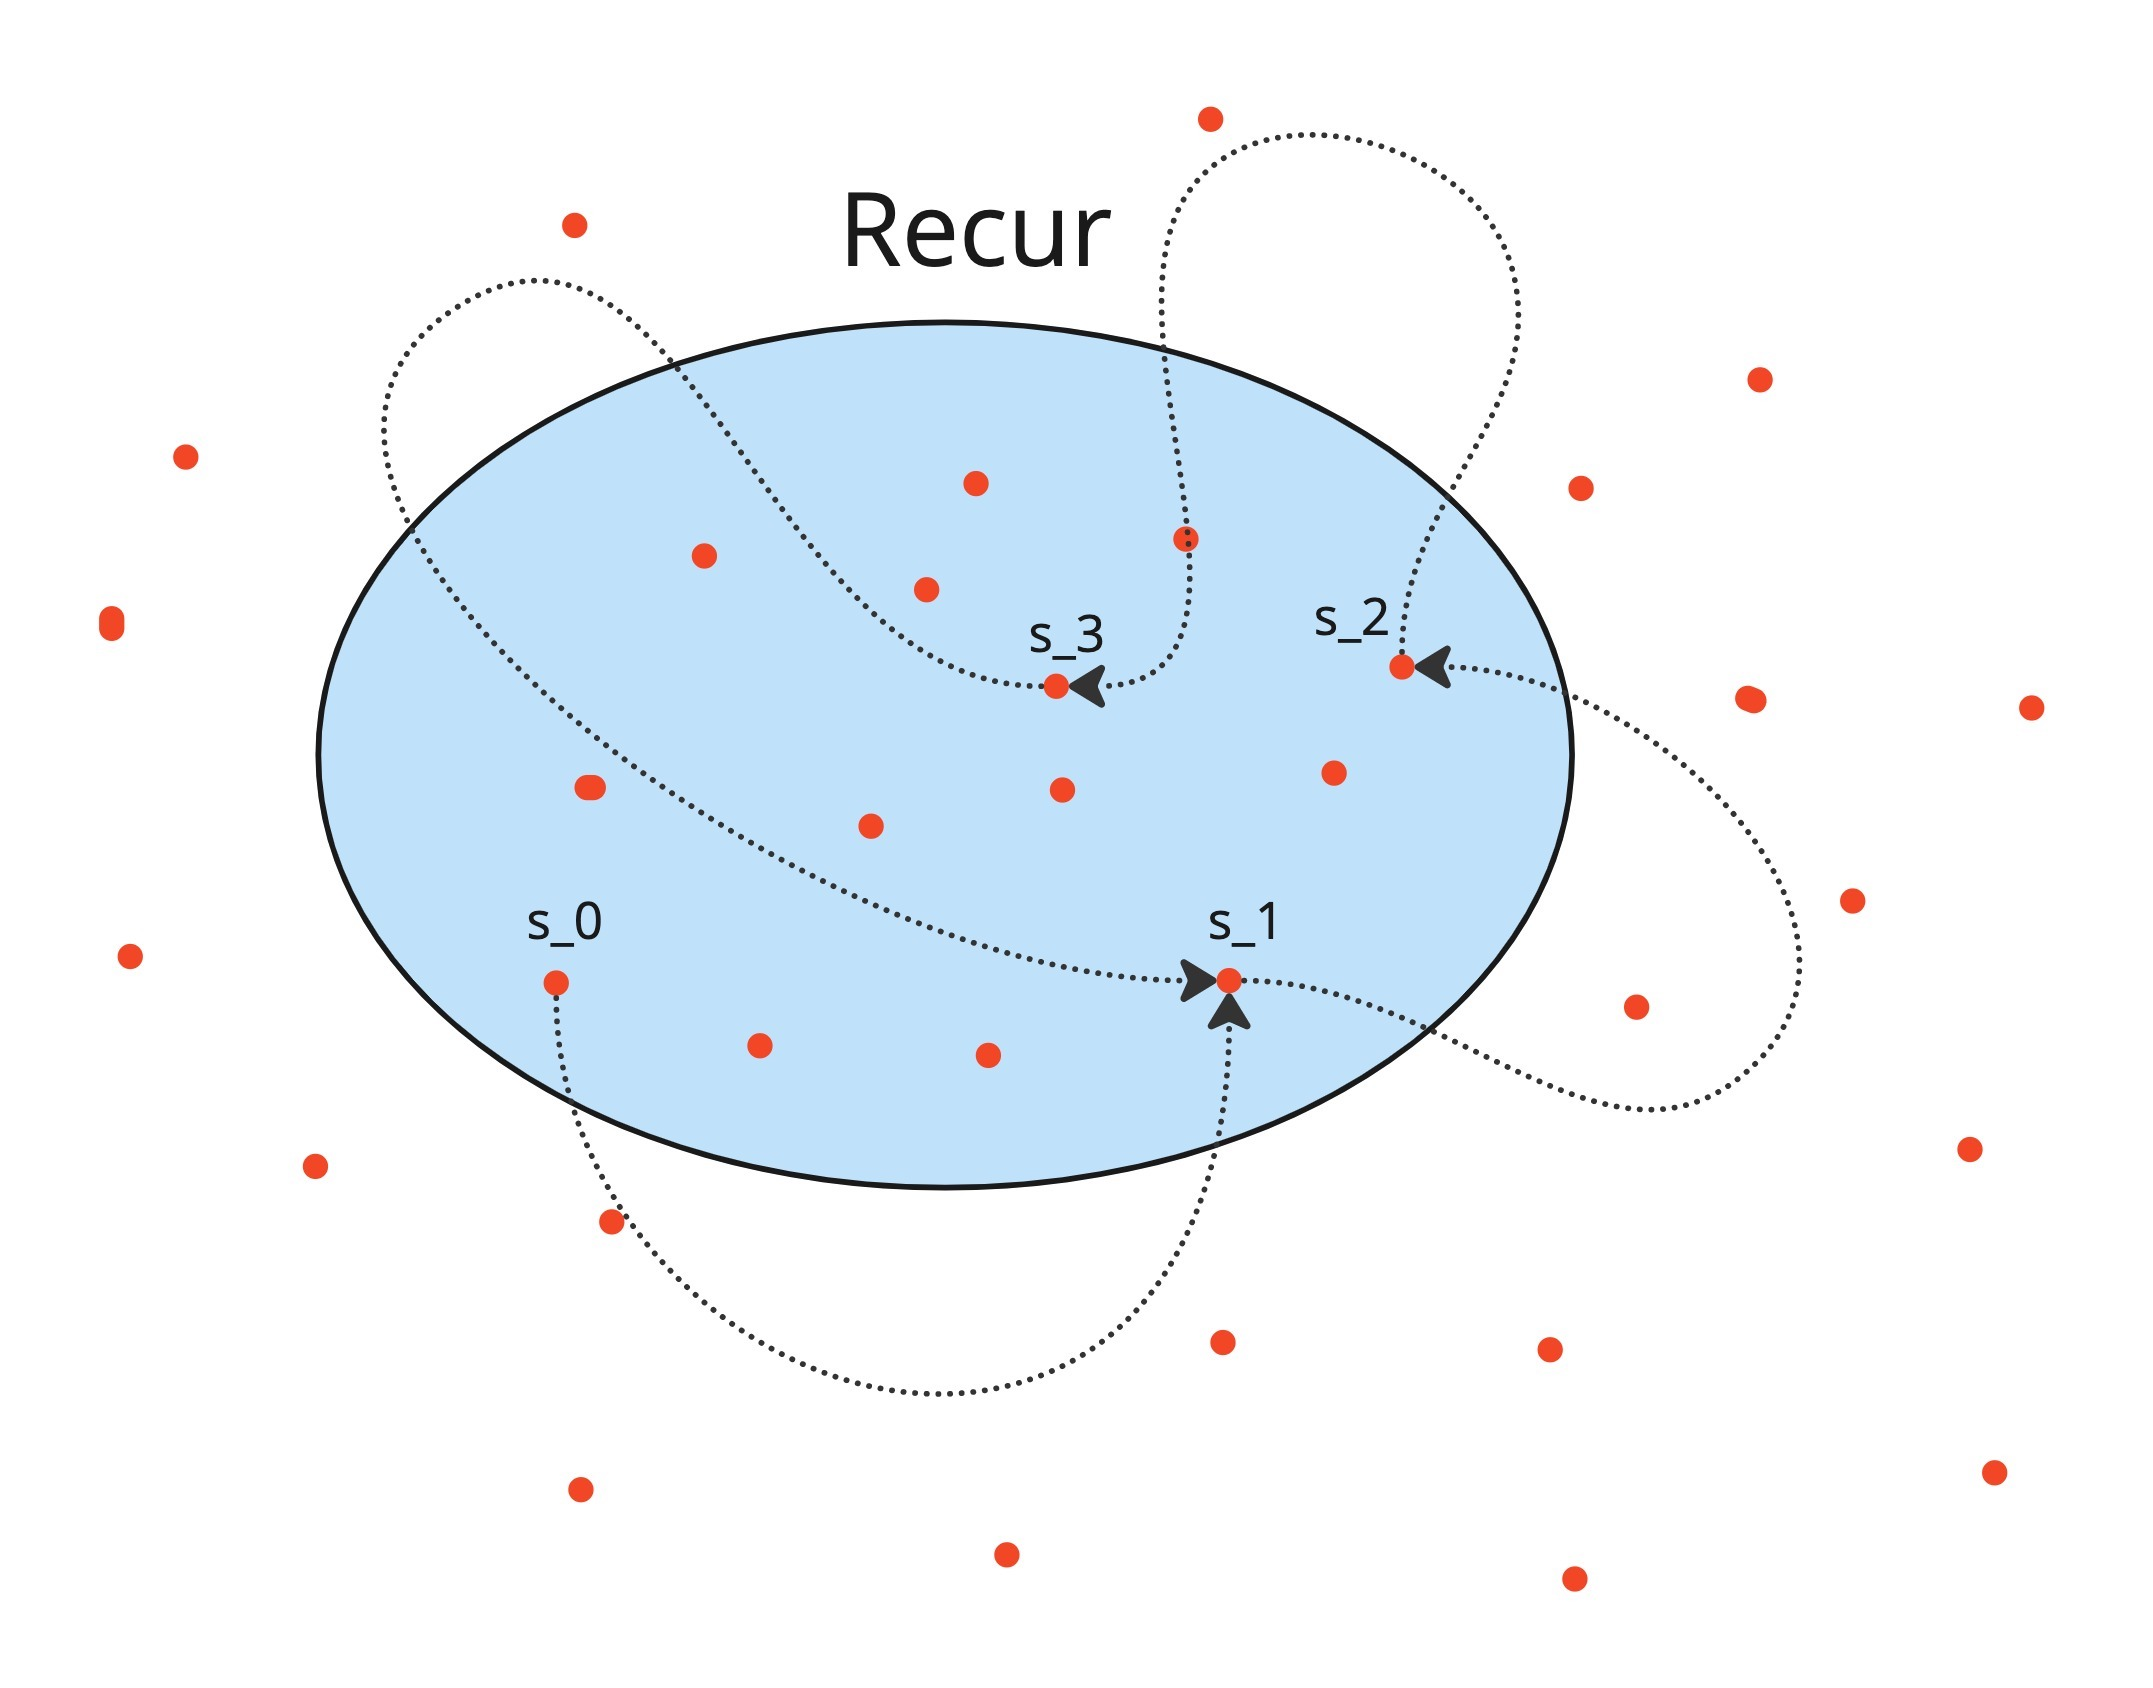
\includegraphics[width=0.6\textwidth]{loop_trace.jpg}
        \caption{Representation of the \texttt{loop\_trace} algorithm.}
        \label{fig:loop_trace}
    \end{figure}
   
    In Figure \ref{fig:loop_trace} each red dot represents a state; each dotted arrow represents the result of a call to \texttt{partial\_loop\_trace}.
    The last part of \texttt{loop\_trace} removes the subpath between \texttt{s\_0} and \texttt{s\_1}.

    \paragraph*{\texttt{init\_to\_s\_trace}}
    This function iteratively computes the reachable region from $Init$ until it finds a path to the given state.
    At each iteration it keeps track of the regions it's going through.
    Finally, it desimbolifies that list in order to return a path from a state in $Init$ to the given state.

    \begin{figure}[H] 
        \centering
        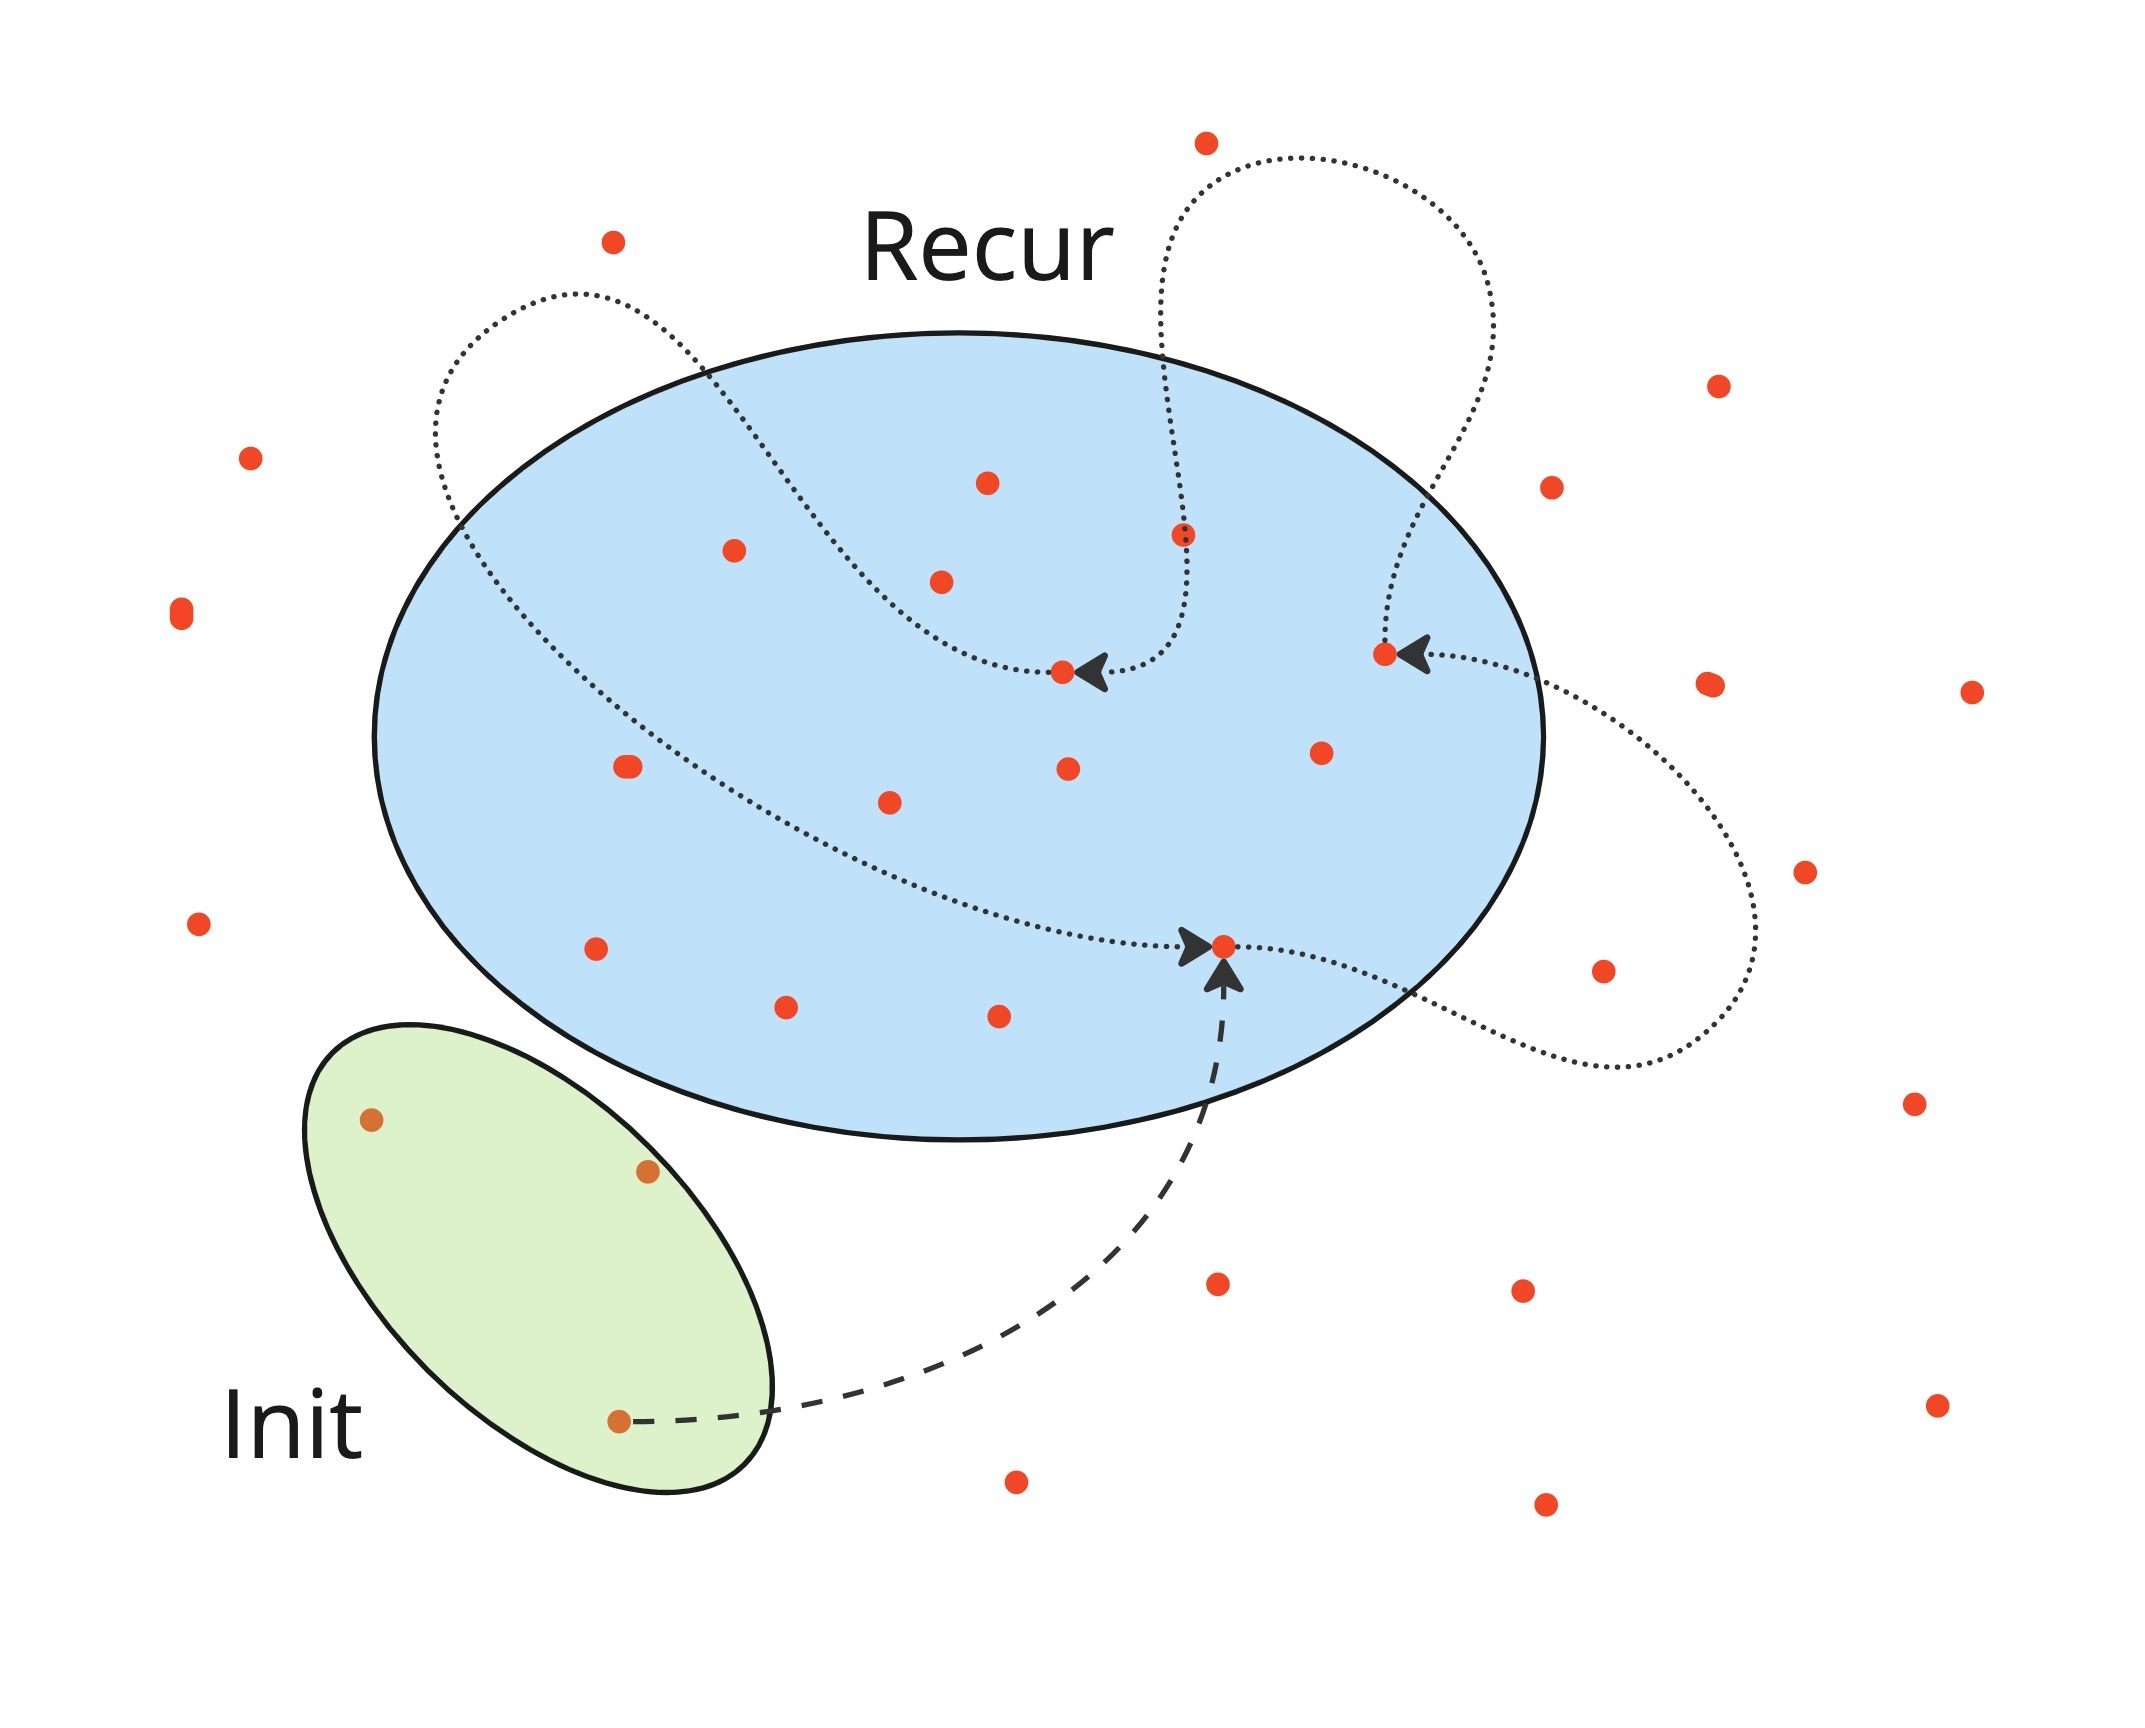
\includegraphics[width=0.6\textwidth]{create_trace.jpg}
        \caption{Representation of the \texttt{create\_trace} algorithm.}
        \label{fig:create_trace}
    \end{figure}

    In Figure \ref{fig:create_trace} each red dot represents a state; the dotted path represents the result of a call to \texttt{loop\_trace}; the dashed arrow represents the result of a call to \texttt{init\_to\_s\_trace}.

    \subsection{Implementation}
    \begin{code}{function that finds a list of states starting from a given state in $Recur$ and ending in $Recur$.}
function partial_loop_trace(s, G, Recur):
    |$New \leftarrow Post(s) \setminus G$|
    |$SymTrace \leftarrow $|[|$s, New$|]
    |$Reach \leftarrow New$|
    while |$New \cap Recur = \nothing$|:
        |$New \leftarrow (Post(New) \setminus Reach) \setminus G$|
        |$SymTrace$| + |$New$|
        |$Reach \leftarrow Reach \cup New$|
    |$SymTrace$|[-1]|$ \leftarrow SymTrace$|[-1]|$ \cap Recur$|
    return desimbolify|$(SymTrace)$|
    \end{code}

    \begin{code}{function that finds a loop starting and ending in the same state in $Recur$.}
function loop_trace(Recur, G):
    |$s \leftarrow$| pick_one_state|$(Recur)$|
    |$Trace \leftarrow$| partial_loop_trace|$(s, G, Recur)$|
    |$s \leftarrow Trace$|.pop|$()$|
    while |$s$| not in |$Trace$|:
        |$Trace \leftarrow Trace$| + partial_loop_trace|$(s, G, Recur)$|
        |$s \leftarrow Trace$|.pop|$()$|
    |$Trace \leftarrow Trace$| + |$s$|
    while |$Trace$|[0]|$ \neq s$|:
        |$Trace \leftarrow Trace$|[1:]
    return |$Trace$|
    \end{code}

    \begin{code}{function that finds a list of states describing a path from $Init$ to a given state.}
function init_to_s_trace(s):
    |$New \leftarrow Init$|
    |$Reach \leftarrow Init$|
    |$Trace \leftarrow $|[|$New$|]
    while |$s \cap New = \nothing$|:
        |$New \leftarrow Post(New) \setminus Reach$|
        |$Reach \leftarrow Reach \cup New$|
        |$Trace + New$|
    |$Trace$|[-1]|$ \leftarrow s \cap New$|
    return desimbolify|$(model, Trace)$|
    \end{code}
\end{document}
